\documentclass{bioinfo}
\copyrightyear{2005}
\pubyear{2005}

\begin{document}
\firstpage{1}

\title[short Title]{This is a title}
\author[Sample \textit{et~al}]{Corresponding Author\,$^{1,*}$, Co-Author\,$^{2}$ and Co-Author\,$^2$\footnote{to whom correspondence should be addressed}}
\address{$^{1}$Department of XXXXXXX, Address XXXX etc.\\
$^{2}$Department of XXXXXXXX, Address XXXX etc.}

\history{Received on XXXXX; revised on XXXXX; accepted on XXXXX}

\editor{Associate Editor: XXXXXXX}

\maketitle


\begin{abstract}

\section{Summary:}
 Numerous methods have been proposed to find the optimal partition of a signal in a given number of segments, but very few address the question of the quality of the segmentation. In many biological data-sets (CGH-array, NGS, ...),  each segment is assumed to be related to a biological event. Thus it is crucial to have precise idea of the uncertainty on the number and position of the segments.
%so that the certainty of their location and the number of segments is crucial. 
EBS is an R package that provides through a Bayesian framework exact quantities such as the posterior distribution of a change-point position, and an efficient ICL criterion for the selection of the total number of change-points. All quantities are computed in a quadratic time.


\section{Availability:}
EBS is available as an R package from CRAN repositories (e.g. http://cran.r-project.org/web/packages).


\section{Contact:} alice.cleynen@agroparistech.fr
\end{abstract}

\section{Introduction}

 Most change-point detection strategies do not address crucial questions like the quality of the segmentation or the uncertainty on the localisation of breakpoints that are useful when choosing the number of segments, or comparing the segmentation of different profiles. 

Among the few are the implementation of Bardy and Hartigan's Bayesian approach (bcp) that uses MCMC approximation, \citep{barry_hartigan, bcp_package}, and the frequentist forward-backward algorithm of \cite{guedon_2008} and constrained-HMM framework of  \cite{Luong_HMM_2012}. Those two later approaches compute those useful quantities for fixed values of the segment parameters.

EBS is an implementation of the framework described in \cite{rigaill_exact_2011} which derives \textbf{exact} posterior probabilities of quantities such as the number of segments, the entropy of a segmentation, or the localisation of the change-points.

The general change-point detection model can be stated as
  follows. Consider data ordered along genomic positions (or probe
  location) $Y = (Y_1, Y_2, \dots Y_n)$. The whole chromosome is
  shattered into successive segments $r$. The observations come from
  some parametric distribution $F$. The parameter depends on the
  segment the observation belongs to: $i \in r \: \Rightarrow \: Y_i
  \sim F(\theta^r)$.
\begin{methods}

\section{Available Functionality}
Our approach is valid for all models satisfying the following factoriability
assumption: if $Y$ denotes the data, $m$ a segmentation and $r$ a
segment of $m$,
\begin{equation}
 (H)\quad P(Y,m) = C \prod_{r\in m} a_r P(Y^r|r) \label{factoriability}
\end{equation}
where $P(Y^r|r) =\int P(Y^r|\theta_r)P(\theta_r)d\theta_r $.

The
package includes the Poisson, Normal Heteroscedastic and Negative
Binomial (with known overdispersion parameter) models that all verify
$(H)$. Normal distribution are dedicated to arrayCGH, whereas Poisson and negative binomial are proposed for NGS.

The computation of the quantities of interest rely on the knowledge of $P(Y,K)$
($K$ being the number of segments) that can be computed in quadratic
time as
\begin{equation}
 P(Y,K) = \left[{n-1} \choose{K-1} \right]^{-1} \left(A^K \right)_{1,n+1} \label{Proba}
\end{equation} 
where $A_{i,j}=P(Y^r)$ where $r$ stands for the segment $[\![i,j[\![$. (See Proposition 2.2 of \cite{rigaill_exact_2011} for proof).


Table \ref{Tab:01} gives the list of the functions available in the EBS Package. This section describes and illustrates their use with a continued example. 

\subsection{Matrix Construction}

All quantities of interest can be computed using simple operations on the elements of the matrix $A$ of segment probabilities. The function \texttt{EBSegmentation} initializes this matrix with the data according to the user's choice of maximum number of segments and data-model. Each of them is associated with a prior distribution on the parameters (for instance, Gamma for the Poisson model), and the result depends on the value of the hyperparameters. By default \texttt{EBSegmentation} uses values such that the prior is non-informative, but the user has the possibility of giving his own hyperparameters.

The function returns an object of class \textit{EBS} which contains the prior information, matrix $A$ and the two matrices $Li$ and $Col$
 which $k^{th}$ row (respectively column) is the first row (resp last column) of the $k^{th}$ power of $A$ ($1\leq k \leq K_{max}$). 
In other words we have: $Li_{i,j}=P([\![Y_0,Y_j[\![,i)$ and $Col_{i,j}=P([\![Y_i,Y_{n+1}[\![,j)$.

\begin{verbatim}
> set.seed(1)
> require(EBS)
> x<-c(rpois(125,1),rpois(100,5),rpois(50,1),
  rpois(75,5),rpois(50,1))
> out <- EBSegmentation(x,Kmax=20)
\end{verbatim}


\begin{table}[!t]
\processtable{Functions provided by EBS package \label{Tab:01}}
{\begin{tabular}{ll}\toprule
Function Name & Output \\\midrule
 EBSegmentation & Initializes matrix $A$ and its $K_{max}$ first powers\\
 EBSBIC & Computes BIC and chooses optimal value of K \\
 EBSICL & Computes ICL and chooses optimal value of K \\
 EBSPostK & Returns the posterior probability of the number of segments\\
 EBSDistrib & Computes the distribution of a change-point\\
 EBSPlotProba & Plots distribution of all change-points for a given K\\\botrule
\end{tabular}}{}
\end{table}




\subsection{Model Selection}

EBS Package provides two model selection criteria:
\begin{itemize}
\item an exact BIC criterion
\item an ICL criterion
\end{itemize}


These criteria can be called with functions \texttt{EBSBIC} and \texttt{EBSICL}. 

Considering the segmentation as an unobserved variable, we can use the ICL criterion introduced by \cite{biernacki_assessingmixture_2000} in the context of incomplete data models to select the number of segments. 
The ICL can be written as $ICL(K) = -\log P(Y,K) + \mathcal{H}(K) \label{ICL}$ where
the entropy $\mathcal{H}(K)$ is defined as :
\begin{equation}
  \mathcal{H}(K)=-\log \sum_{m\in \mathcal{M}_K} p(m|Y,K) \log p(m|Y,K)
\end{equation}
The entropy can be viewed as a penalty term and it is computed in a quadratic time. 
 Even though in this context the Bayesian Information Criterion is exact, it overestimates the number of segments while the ICL performs better \citep{rigaill_exact_2011}. However, the computation of the BIC (through function \texttt{EBSPostK}) can be usefull for later analysis such as Bayesian Model Averaging (BMA).
\begin{verbatim}
> bic <- EBSBIC(out)
> print(bic$NbBIC)
[1] 9
> icl <- EBSICL(out)
> print(icl$NbICL)
[1] 5

\end{verbatim}


\begin{figure}[!h]%figure1
\centerline{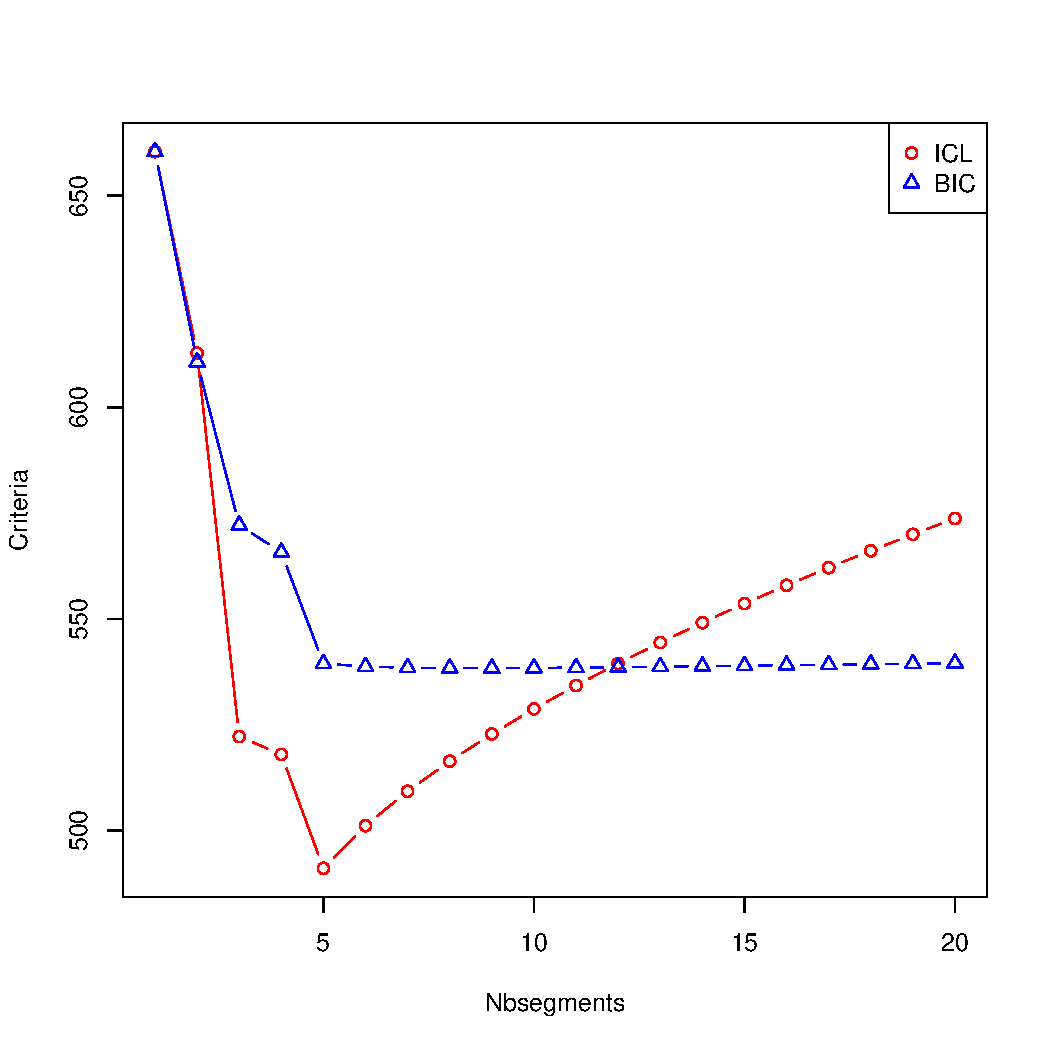
\includegraphics[width=4.5cm]{icl-bic.pdf}}
\caption{BIC and ICL criteria as a function of the number of segments} \label{fig:01}
\end{figure}






\subsection{Change-point location distribution}

Once the number of segments is chosen, one might be interested in the distribution of the location of each change-points. Two functions are implemented to address this question. \texttt{EBSDistrib} returns the distribution of the $k^{th}$ changepoint of a segmentation in $K$ segments. \texttt{EBSPlotProba} plots the distribution of all $K\!-\!1$ change-points of a segmentation in $K$ segments. The user has the option to plot those distributions on top of the data. 
\begin{verbatim}
> EBSPlotProba(out, Kicl, data=TRUE,
  file="my-segmentation.pdf")
\end{verbatim}

Figure \ref{fig:02} shows the output. 

\begin{figure}[!h]%figure1
\centerline{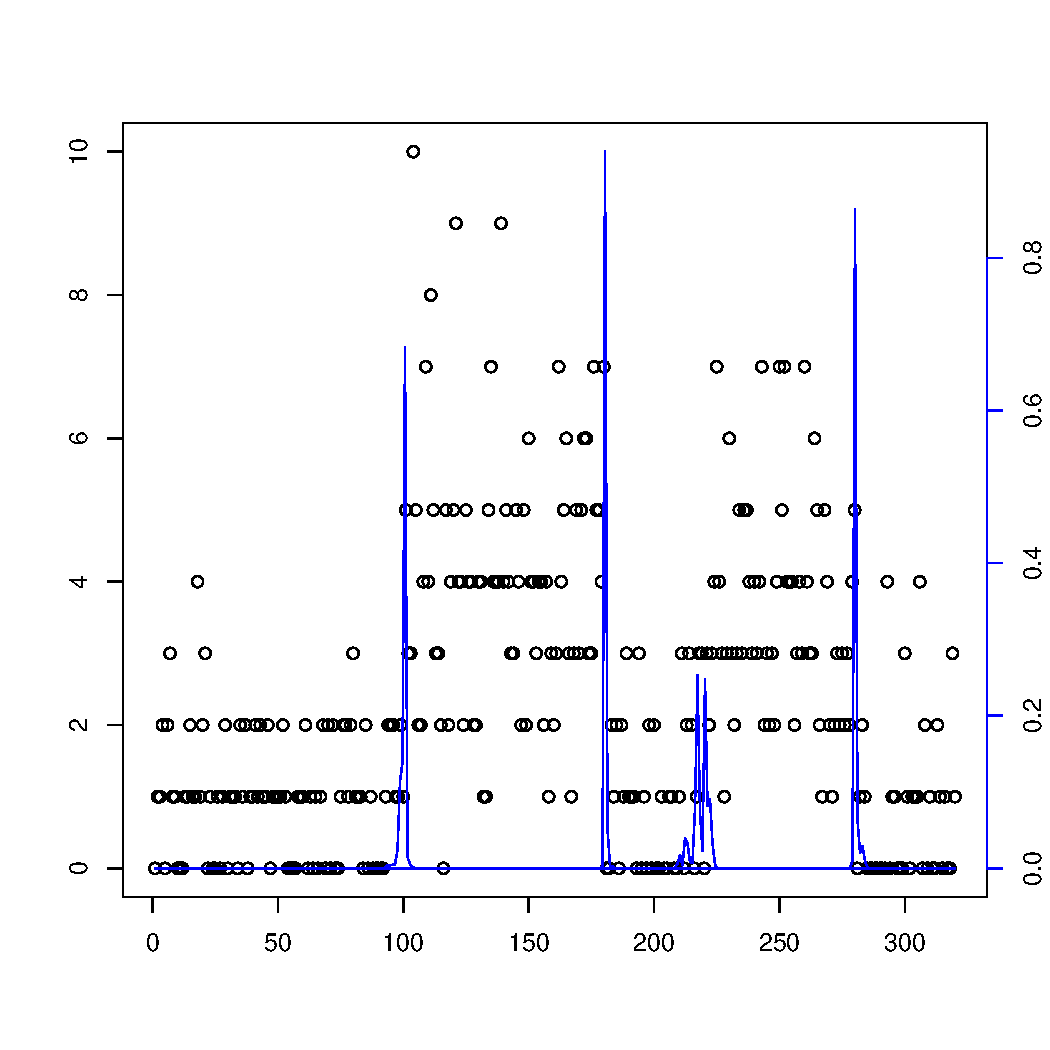
\includegraphics[width=6cm]{my-segmentation.pdf}}
\caption{file \textit{my-segmentation.pdf}, output of function \texttt{EBSPlotProba}}\label{fig:02}
\end{figure}




\section{Conclusion}

This note introduces the EBS package for the analysis of NGS and CGH-array data. It allows a complete analysis of the segmentation space for biological profiles in an exact Bayesian framework. 
It provides an efficient criterion for the selection of the number of segments and allows further analysis of variables such as the entropy or the location of a change-point. 
Future improvements of the package include the analysis of other quantities of interest such as the posterior mean of the signal.



\section*{Acknowledgement}
We whish to thank Gregory Nuel and Michel Koskas for their help dealing with numerical issues.


%\bibliographystyle{natbib}
%\bibliographystyle{achemnat}
%\bibliographystyle{plainnat}
%\bibliographystyle{abbrv}
%\bibliographystyle{bioinformatics}
%
%\bibliographystyle{plain}
%
%\bibliography{Document}


\begin{thebibliography}{}

\bibitem[Barry and Hartigan, 1993]{barry_hartigan} Barry, D., and Hartigan, J. A. (1993) A Bayesian Analysis for Change Point Problems {\it Journal of the American Statistical Association}, {\bf 88} 309-319

\bibitem[Biernacki {\it et~al}., 2000]{biernacki_assessingmixture_2000} Biernacki, C., Celeux, G. and Govaert, G. (2000) Assessing a mixture model for clustering with the integrated completed likelihood, {\it{IEEE} Transactions on Pattern Analysis and Machine Intelligence}, {\bf 22} 719-725.

\bibitem[Erdman and Emerson, 2007]{bcp_package}   Chandra Erdman and John W. Emerson (2007) {\bf{bcp}}: An {R} Package for Performing a Bayesian Analysis
      of Change Point Problems {\it Journal of Statistical Software}, {\bf 3} 1-13

\bibitem[Guedon, 2008]{guedon_2008} Guédon, Y. (2008) Explorating the segmentation space for the assessment of multiple change-points models. {\it Technical report, Preprint INRIA} {\bf 6619}

\bibitem[Luong {\it et~al}, 2012]{Luong_HMM_2012} Luong, T.~M., Rozenholc, Y. and Nuel, G. (2012) Fast estimation of posterior probabilities in change-point models through a constrained hidden Markov model {http://adsabs.harvard.edu/abs/2012arXiv1203.4394L}.

\bibitem[Rigaill {\it et~al}., 2010]{rigaill_exact_2011} Rigaill, G., Lebarbier, E., Robin, S. (2011) Exact posterior distributions over the segmentation space and model selection for multiple change-point detection problems, {\it Statistics and Computing}, {\bf 22-4}, 917-929.

\end{thebibliography}
\end{methods}
\end{document}
